%\usepackage{xr}

% \externaldocument{note01}
% \externaldocument{note02}
% \externaldocument{note03}
% \externaldocument{note04}
% \externaldocument{note05}
% \externaldocument{note06}
% \externaldocument{note07}
% \externaldocument{note08}
% \externaldocument{note09}
% \externaldocument{note10}
% \externaldocument{note11}

\graphicspath{{./input/graphs/note04/}}


% \zexternaldocument{note01}
% \zexternaldocument{note02}
% \zexternaldocument{note03}
% \zexternaldocument{note04}
% \zexternaldocument{note05}
% \zexternaldocument{note06}
% \zexternaldocument{note07}
% \zexternaldocument{note08}
% \zexternaldocument{note09}
% \zexternaldocument{note10}
% \zexternaldocument{note11}
% \externaldocument{note12}


\week{4}
\lecture{10}{Analyticity and other...}
% \section*{Week 4. Lecture 10}

We have studied the continuity and differentiability of complex functions. Our next subject - analytic functions.

\section{Single-valued analytic functions.}

Recall: If for any $z$ corresponds one value $f(z)$, then we say that $f$ is single-valued function.

\subsection{Definitions and examples}

\begin{definition}\label{definition:7.1} Single-valued function $f(z)$ is analytic at the 
    point $z_0$ if there exists $\epsilon$-neighborhood $D(z_0, \epsilon)$ of $z_0$ so that $f$ is differentiable at every $z \in D(z_0, \epsilon)$.
\end{definition}
We have proved that if $f$ is differentiable at $z_0$, then $f$ is continuous at $z_0$, therefore if $f$ is analytic at $z_0$, then $f$ is continuous at $z_0$.

Let us note that we will also use names Holomorphic or Regular functions for analytic functions.

\begin{definition}\label{definition:7.2} A function that is analytic for every $z \in \mathbb{C}$ (on the whole plane) is called an entire function.
\end{definition}
\begin{definition}\label{definition:7.3} Single-valued function is analytic on a domain (open connected subset of the plane $\mathbb{C}$) $\Omega$ if it is differentiable at every $z \in \Omega$.
\end{definition}
Note: From Def~\ref{definition:7.1}: a set on which the function is analytic needs to be open, 
however if we say that some function $f$ is analytic in a closed set, we mean that there exists an open set that 
contains this closed set and the function is analytic on this open set.

\begin{example}\label{example:9.1}
    Polynomial $P_n(z) = a_0 + a_1z + \dots + a_nz^n$ - single-valued function differentiable at every $z \in \mathbb{C} \implies$ analytic on $\mathbb{C} \implies$ entire.
\end{example}

\begin{example}\label{example:9.2}
    Every rational function $f(z) = \frac{P_n(z)}{Q_m(z)}$ where $P_n(z), Q_m(z)$ are polynomials 
    (of deg $n, m$ respectively) without common factors is analytic on $\mathbb{C}$ except for the roots of $Q_m(z)$, 
    namely except for the points where $Q_m(z) = 0$. For instance: $f(z) = \frac{z-1}{z^2 + iz} = \frac{z-1}{z(z+i)}$ is analytic everywhere except for $z = 0, -i$. 
    For example, it is analytic on the following domains:
% \begin{align*}
    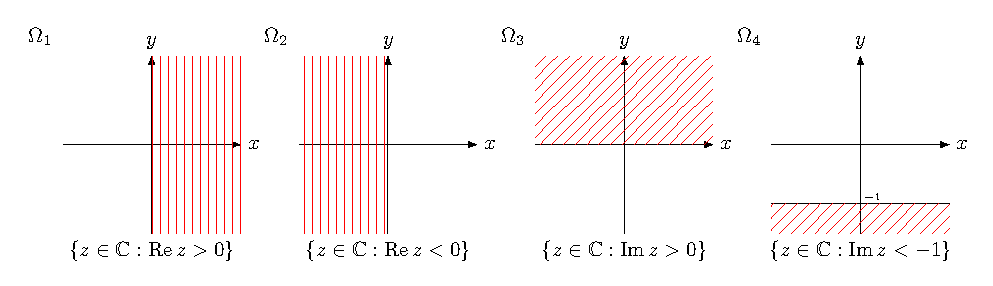
\includegraphics[width=\textwidth]{image_graph1.pdf}

    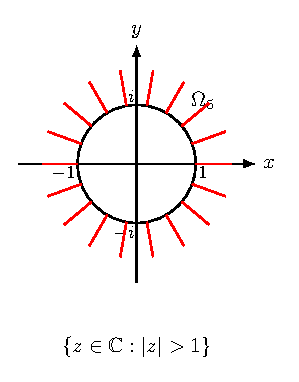
\includegraphics{img_graph2.pdf}

    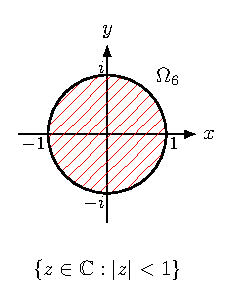
\includegraphics{img_graph3.pdf}
% \end{align*}
$\{z \in \mathbb{C}: \text{Re } z > 0\} \quad \{z \in \mathbb{C}: \text{Re } z < 0\} \quad \{z \in \mathbb{C}: \text{Im } z > 0\} \quad \{z \in \mathbb{C}: \text{Im } z < -1\}$

But it is not analytic in $\Omega_6$, since $\partial \in \{z \in \mathbb{C}: |z| < 1\}$ and $f$ is not defined at $z = 0$.

$\{z \in \mathbb{C}: |z| > 1\} \quad \{z \in \mathbb{C}: |z| < 1\}$
\end{example}

Note: $f$ is analytic on a domain $\Omega \iff u$ and $v$ are differentiable on $\Omega$ and CR equations hold.

Exercise (Ex 9.3) The function $f(z) = e^x \cos y + ie^x \sin y = e^z$ is entire.

In the next example: a function for which CR equations hold on the whole plane, but $u$ and $v$ are \emphw{not} differentiable on the whole plane, thus the function is \emphic{not}{} entire.

\begin{example}\label{example:9.4}
\[ 
f(z) = \begin{cases}
e^{-1/z^4} & z \neq 0 \\
0 & z = 0
\end{cases}
\text{ defined everywhere in } \mathbb{C} 
\]

\checkthis CR equations hold for every $z \in \mathbb{C}$.
\end{example}
Claim:
\begin{claim} $f(z)$ is not continuous at $z = 0$ ($\implies$ not differentiable).

    \begin{proof}
 Compute $\lim_{z \to 0} f(z)$ on the path $y = x$:
\[ \lim_{\substack{x \to 0 \\ y = x}} e^{-\frac{1}{(x+iy)^4}} = \lim_{x \to 0} e^{-\frac{1}{(1+i)^4 x^4}} = \lim_{x \to 0} e^{\frac{1}{4x^4}} = +\infty \]
$(1 + i)^4 = (\sqrt{2})^4 (\cos(\frac{\pi}{4}) + i\sin(\frac{\pi}{4})) = -4$ De Moivre.
    \end{proof}
\end{claim}
Next proposition is analogous to propositions about the limits, continuity, and differentiability.

\subsection{Properties of analytic functions}

\begin{proposition}\label{proposition:7.1} If $f, g$ are analytic functions on a domain $\Omega$, then also $f + g$ and $f \cdot g$ are analytic on $\Omega$. If $g(z) \neq 0$ on $\Omega$, then $\frac{f}{g}$ is analytic on $\Omega$. The composition $(g \circ f)$ of two analytic functions on $\Omega$ is an analytic function on $\Omega$.

\begin{proof} \emphi{EXERCISE} \end{proof}
\end{proposition}
\begin{example}\label{example:9.5}
    Prove: if $f(z)$ is analytic and real on a domain $\Omega$, then $f$ is a constant function.

\begin{proof} $f$ is analytic and real on $\Omega \implies f(x,y) = u(x,y) + i \cdot 0$, namely $v(x,y) = 0$; CR equations hold for every $z \in \Omega$.
$f$ from analyticity on $\Omega$: $\frac{\partial u}{\partial x} = \frac{\partial v}{\partial y} = 0$ and 
$\frac{\partial u}{\partial y} = -\frac{\partial v}{\partial x} = 0 \implies u(x,y) = c \in \mathbb{R} \implies f(x,y) = c$, namely $f$ is a constant function.
\end{proof}
\end{example}
\begin{proposition} \label{proposition:7.2}
    If $f$ is analytic on a domain $\Omega$ and $f'(z) = 0$ for all $z \in \Omega$, then $f$ is constant on $\Omega$.

\begin{remark}
     Prop 7.2 is false if $\Omega$ is not connected - $f$ can take different constants (constant values) on each connected component of $\Omega$.
\end{remark}
\begin{proof}
    The version of this proposition for real functions is proved using the Mean Value Theorem, 
    that asserts that under appropriate continuity assumption for $f: (a,b) \to \mathbb{R}$ there exists $c \in (a,b)$ s.t. $f(b) - f(a) = f'(c)(b-a)$. 
    So, if $f'(x) = 0$ for all $x \in (a,b)$, then $f(b) = f(a)$. The problem in the complex case is that there is no analogous idea of "between $a$ and $b$" in $\mathbb{C}$, 
    since there are many routes from $a$ to $b$.

    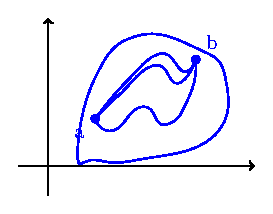
\includegraphics{img_graph4.pdf}

However, we can use the Mean Value Theorem for Re $f$ and Im $f$ as follows:

Since $f'(z) = 0$ for all $z \in \Omega$ by CR equations $0 = f'(z) = \frac{\partial u}{\partial x} + i\frac{\partial v}{\partial x}$ for all $z \in \Omega \implies \frac{\partial u}{\partial x} = \frac{\partial u}{\partial y} = \frac{\partial v}{\partial x} = \frac{\partial v}{\partial y} = 0$ for all $z \in \Omega$.
\end{proof}

\begin{claim} $u$ is a constant function.
    \begin{proof}
        We have $u: \Omega \to \mathbb{R}, \frac{\partial u}{\partial x} = \frac{\partial u}{\partial y} = 0$ for all $(x,y) \in \Omega$. Pick $(x_0, y_0), (x_1, y_1) \in \Omega$. $\Omega$ is connected, 
        thus by Def~\ref{definition:4.2} any 2 points in $\Omega$ can be connected by a path that is entirely in $\Omega$. 
        We join $(x_0, y_0)$ and $(x_1, y_1)$ by a path comprised of pieces parallel to $x$-axis or 
        $y$-axis [One needs to show that such path exists!] 
        Since $\frac{\partial u}{\partial x} = 0$ by the Mean Value Theorem, $u$ is constant on the horizontal pieces. In the same way,
        since $\frac{\partial u}{\partial y} = 0$, $u$ is constant on vertical pieces. Thus, $u$ is constant on $\Omega$.
        By a similar argument we obtain that $v$ is constant on $\Omega$, therefore $f = u + iv$ is constant on $\Omega$.
    \end{proof}
\end{claim}
\end{proposition}

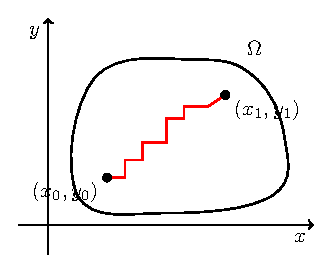
\includegraphics{img_graph5.pdf}

Now we are going to study analyticity of multi-valued functions - here we will see the big difference between the complex and real functions.

\section{Analyticity of multi-valued functions}

\subsection{Branch points and branches}
We have seen that analytic function is always continuous, thus multi-valued functions are not analytic as is. The question is: can we choose a branch of such function that is single-valued and analytic?

\begin{definition}\label{definition:8.1} We say that on a domain $\Omega$ there is a single-valued 
    branch of multi-valued function if for every point of $\Omega$ we can choose one of the values of a function such that the resulting single-valued function is continuous in $\Omega$.
\end{definition}

In other words: to choose single-valued branch means to choose the domain of definition of a function such that when a point $z$ 
moves along some closed continuous curve that is contained in the domain of definition and goes back to the starting point we get the same value of the function.

Let us demonstrate how we do that on the following example.

\begin{example}\label{example:10.1} 
    Consider double-valued function $f(z) = \sqrt{z - z_0}$. $f(z)$ is defined for all $z \in \mathbb{C}$. Write: $z - z_0 = r(\cos \theta + i\sin \theta), r = |z - z_0|, \theta = \arg(z - z_0)$.

At every $z \neq z_0$, $f(z)$ attains 2 values ($\implies$ double-valued!).
\begin{align*}
    w_0 &= \sqrt{r}\left(\cos \frac{\theta}{2} + i\sin \frac{\theta}{2}\right) \\
    w_1 &= \sqrt{r}\left(\cos\left(\frac{\theta}{2} + \pi\right) + i\sin\left(\frac{\theta}{2} + \pi\right)\right) = -\sqrt{r}\left(\cos \frac{\theta}{2} + i\sin \frac{\theta}{2}\right) = -w_0
\end{align*}

Let us follow the value $w_0$ when $z$ is on the closed continuous curve $L$ that encircles $z_0$ counterclockwise (anti-clockwise; the positive direction).

If $z$ moves to $z_1$, the argument of $z_1 - z_0$ will be
$\arg(z_1 - z_0) = \theta + \theta_1$.

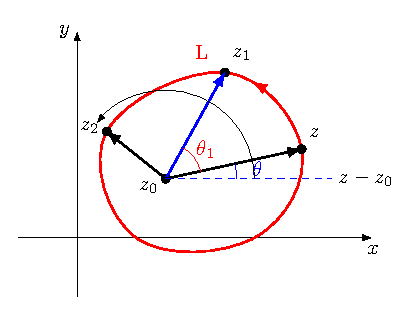
\includegraphics{img_graph6.pdf}

If it continues to move along $L$, $z$ will eventually return to the starting point: the modulus $r = |z - z_0|$ will be the same, 
but the argument will increase by $2\pi$ (since we completed the circle), and $w_0$ will attain the new value $w_1$.
\begin{align*} 
    w_{new} & = \sqrt{r}\left(\cos\left(\frac{\theta + 2\pi}{2}\right) + i\sin\left(\frac{\theta + 2\pi}{2}\right)\right) \\ 
            & = \sqrt{r}\left(\cos\left(\frac{\theta}{2} + \pi\right) + i\sin\left(\frac{\theta}{2} + \pi\right)\right) = w_1 = -w_0 
\end{align*}

Let us check what happens to $w_0$ is we move along a closed continuous curve that does not encircle the point $z_0$.
\end{example}

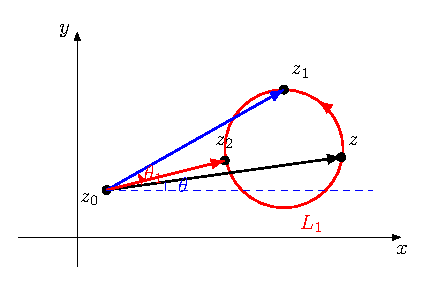
\includegraphics{img_graph7.pdf}

From the picture above that the value of the modulus and of the argument after completing the full circle will return to its starting value - the same, with no change. 
This is independent of the curve $L_1$ (the only important thing that the curve does not encircle the point $z_0$).
\begin{corollary}\label{corollary:8.1} 
    On a domain $\Omega$ that contains curves that encircle $z_0$, it is impossible to choose a continuous branch of the function $\sqrt{z - z_0}$.
\end{corollary}

% \section*{Lecture Notes,Lectures 11 + 12}
\lecture{11+12}{Continuation and Harmonic functions}

We have studied the double-valued function \( f(z) = \sqrt{z - z_0} \).

Reference, corollary \ref{corollary:8.1}.

For example: On \( \frac{1}{2} < |z - z_0| < 2 \), it is impossible to choose a single-valued branch of \( \sqrt{z - z_0} \).

On \( |z - z_0| > 1 \), it is impossible to choose a single-valued branch of \( \sqrt{z - z_0} \).

We have also seen that if the curve does not encircle \( z_0 \), then the value of \( \sqrt{z - z_0} \) stays the same. 
So, we have another corollary.

\begin{corollary}\label{corollary:8.2}
    It is possible to choose a single-valued branch of the function \( \sqrt{z - z_0} \) on a domain \( \Omega \) 
    if none of the closed continuous curves in \( \Omega \) encircle \( z_0 \).
\end{corollary}

Intuitively, if we would be able to "cut" the plane (in some way) up to \( z_0 \), including \( z_0 \), then there will be no closed curve that encircles \( z_0 \).
Indeed, the biggest domain on which none of the closed continuous curves encircle \( z_0 \) is the cutted plane, where we cut as follows.

\subsection*{The "largest" such domain}
\begin{itemize}
    \item Cut-plane: \( \mathbb{C} \) without the line \( \{ z = x + iy \mid x \leq x_0 \} \) 
    (including \( z_0 \)).
    
    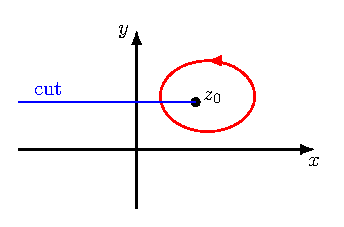
\includegraphics{img_graph8.pdf}

    \item Cut-plane: two single-valued branches:
    \[
        w_0 = \sqrt{r} (\cos \frac{\theta}{2} + i \sin \frac{\theta}{2}), \quad 
        w_1 = -\sqrt{r} (\cos \frac{\theta}{2} + i \sin \frac{\theta}{2})
    \]

    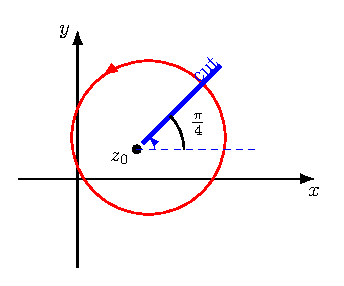
\includegraphics{img_graph9.pdf}
\end{itemize}

\emphOnly{Note}: We can cut along any ray starting at \( z_0 \).

The cut will prevent any closed curve from encircling \( z_0 \). In the case of the line in the picture above (ray creates an angle \( \theta \) with the positive counterclockwise direction with the \( x \)-axis), we have:

For a ray with \( \theta = \frac{\pi}{4} \), two continuous branches of \( \sqrt{z - z_0} \):

\[
    w = \pm \sqrt{r} (\cos \frac{\theta}{2} + i \sin \frac{\theta}{2}), \quad \frac{\pi}{4} < \theta \leq \frac{5\pi}{4}
\]

\begin{definition}\label{definition:8.2} The point \( z_0 \) is called a \textit{branch point} for a complex multi-valued function if the value of \( f(z) \) does not return to its initial value as a closed curve around the point is traced (starting from some arbitrary point on the curve) in such a way that \( f \) varies continuously as the path is traced.
\end{definition}
\textbf{Important:} What matters here is the \textbf{local} behavior of the function \( f \) near \( z_0 \). What may happen on paths that are some distance away from \( z_0 \) is not relevant. To be more precise:

\noindent \textbf{The behavior must occur for all the curves that enclose the point and are sufficiently close to it.}

In example \ref{example:10.1} \( z = z_0 \) is the \textbf{Branch Point}.

Let us consider a more general case.


\begin{example} Consider \( w = \sqrt[n]{z - z_0} \). Take \( z - z_0 = r (\cos \theta + i \sin \theta) \). Then:

\[
w_k = \sqrt[n]{r} \left( \cos \frac{\theta + 2\pi k}{n} + i \sin \frac{\theta + 2\pi k}{n} \right), \quad k = 0,1,2, \dots, n-1.
\]

Fix \( 0 \leq k_0 \leq n-1 \).

As before, we let \( z \) be on the closed continuous curve \( L \) that encloses \( z_0 \). 

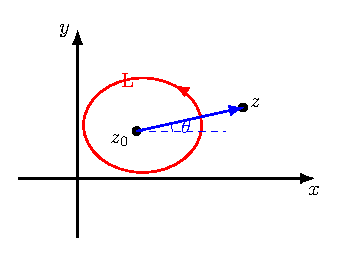
\includegraphics{img_graph10.pdf}

When \( z \) will complete the full circle (anticlockwise), the modulus \( r \) will return to the same value. The argument, however, will increase by \( 2\pi \), and \( w \) will attain a new value.
% \end{example}
\emphic{After full circle around $z_0 $:}{}
\[
w = \sqrt[n]{r} \left( \cos \frac{(\theta + 2\pi) + 2\pi k_0}{n} + i \sin \frac{(\theta + 2\pi) + 2\pi k_0}{n} \right).
\]

\[
= \sqrt[n]{r} \left( \cos \frac{\theta + 2\pi k_0}{n} + i \sin \frac{\theta + 2\pi k_0}{n} \right) 
\cdot \left( \cos \frac{2\pi}{n} + i \sin \frac{2\pi}{n} \right).
\]

\[
= w_{k_0} \left( \cos \frac{2\pi}{n} + i \sin \frac{2\pi}{n} \right) = w_{k_0 + 1}.
\]
\end{example}

Namely, the new value of \( w \) is equal to the previous one times \( \left( \cos \frac{2\pi}{n} + i \sin \frac{2\pi}{n} \right) \).

\checkthis{}

\[
\left( \cos \frac{2\pi}{n} + i \sin \frac{2\pi}{n} \right)^n = 1.
\]

This is independent of the curve that encloses \( z_0 \). If \( z \) runs on a curve that does not encircle \( z_0 \), then, as before, the value \( w_{k_0} \) will not change once \( z \) returns to the starting point.

\textbf{Conclusion:} If \( z \) is on the curve that encloses \( z_0 \) once (anticlockwise), then the value \( \sqrt[n]{z - z_0} = w_{k_0} \) will change to the new value \( w_{k_0 + 1} \). If \( z \) is on the curve that does not enclose \( z_0 \), 
then the value of the function stays the same.
$\implies z = z_0$ is the branch point of the function $f(z) = \sqrt[n]{z - z_0}$.

\begin{example}\label{example:10.3} Find the branch points of the function $f(z) = \sqrt{1 + z^2}$.
    \begin{soln}
        $\sqrt{1 + z^2} = \sqrt{z - i} \cdot \sqrt{z + i}$, therefore $z = \pm i$ are the branch points of $\sqrt{z - i}$, $\sqrt{z + i} \implies$ branch points of $\sqrt{1 + z^2}$.
Let us see on the picture what happens and where to cut so we will be able to obtain a continuous single-valued branch of $f(z)$.

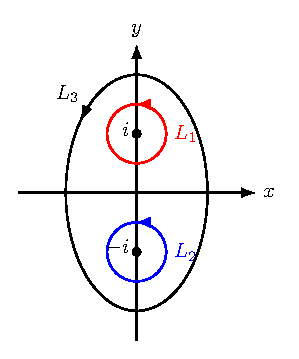
\includegraphics{img_graph11.pdf}

If $z$ is on $L_1$ (around $z = i$): when $z$ returns to the initial point $\sqrt{z + i}$ returns to the same value since $L_1$ does not enclose $z = -i$ while $\sqrt{z - i}$ attains new value - changes the sign of the previous one. Therefore, $f(z)$ also changes the sign. In the same way: if $z$ is on $L_2$, then upon return to the initial point $\sqrt{z + i}$ will change the value - change the sign, $\sqrt{z - i}$ will return to the same value, and the function will change the sign. If $z$ is on $L_3$ that encloses both $z_0 = i$ and $z_0 = -i$, then $\sqrt{z - i}$ and $\sqrt{z + i}$ will change the sign, but their product - the original function - will not!
    \end{soln}
\end{example}

$\implies$ We can choose a continuous branch on a domain $\Omega$ if none of the closed curves in $\Omega$ enclose $i$ and not $-i$ (or $-i$ and not $i$), but it can enclose both. Namely, if we cut the plane along the interval connecting $i$ and $-i$, we will get a domain in which it is possible to choose a continuous branch.

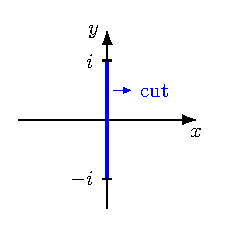
\includegraphics{img_graph12.pdf}

\begin{definition}\label{definition:8.3} Single-valued branch is called an analytic function on a domain $\Omega$ if it is differentiable at every $z \in \Omega$.
\end{definition}

\begin{example}\label{example:10.4} Prove that $w = \sqrt[n]{z}$ is analytic on the domain $\Omega = \{z \in \mathbb{C}: 0 < \arg z < \frac{2\pi}{n}\}$.

\begin{proof}    We have already seen that on the cut-plane with the cut
along any ray starting at $z_0 = 0$ (including $z_0 = 0$) every branch of this function is single-valued and continuous. Let us prove that it is differentiable and find the derivative.

\begin{align*}  & \frac{f(z) - f(z_0)}{z - z_0} = \frac{(f(z))^n - (f(z_0))^n}{z - z_0} \\ 
                & = \frac{1}{(\sqrt[n]{z})^n - (\sqrt[n]{z_0})^n} \cdot \frac{(f(z))^{n-1} + (f(z))^{n-2}f(z_0) + \dots + (f(z_0))^{n-1}}{z - z_0} \\
                & = \frac{1}{(\sqrt[n]{z})^{n-1} + (\sqrt[n]{z})^{n-2}\sqrt[n]{z_0} + \dots + (\sqrt[n]{z_0})^{n-1}} \end{align*}

Now we pass to the limit as $z$ tends to $z_0$ and obtain
\[ \implies \lim_{z \to z_0} \frac{f(z) - f(z_0)}{z - z_0} = \frac{1}{n(\sqrt[n]{z_0})^{n-1}} \]
$\implies f$ is differentiable and \[ (\sqrt[n]{z})' = \frac{1}{n(\sqrt[n]{z})^{n-1}}.\]
\end{proof}
\end{example}

In many problems in hydrodynamics, the elasticity theory and other fields there is often a need to recreate an analytic function from its real part. Now we will find the set of functions for which it is possible. Our subject is:

\section{Harmonic functions.}

\subsection{Definitions and basic results}

\begin{definition}\label{definition:9.1} The real function $u(x,y)$ is called harmonic on a domain $\Omega$ if it is continuous on $\Omega$ with continuous partial derivatives of the first and second order 
    \[\{\frac{\partial u}{\partial x}, \frac{\partial u}{\partial y}, \frac{\partial^2 u}{\partial x^2}, \frac{\partial^2 u}{\partial y^2}, \frac{\partial^2 u}{\partial x \partial y}, \frac{\partial^2 u}{\partial y \partial x}\},\] and the following equation, called the Laplace equation, holds:
\[ \frac{\partial^2 u}{\partial x^2} + \frac{\partial^2 u}{\partial y^2} = 0 \]
\end{definition}

\begin{example}\label{example:11.1} The function $u(x,y) = x^2 - y^2$ is harmonic for every $(x,y) \in \mathbb{R}^2$.
\begin{soln}
         $u(x,y)$ is defined everywhere, and we have:
    $\frac{\partial u}{\partial x} = 2x \quad \frac{\partial u}{\partial y} = -2y \quad \frac{\partial^2 u}{\partial x^2} = 2 \quad \frac{\partial^2 u}{\partial y^2} = -2 \quad \frac{\partial^2 u}{\partial x \partial y} = \frac{\partial^2 u}{\partial y \partial x} = 0$
    
    All partial derivatives are continuous everywhere, and $\frac{\partial^2 u}{\partial x^2} + \frac{\partial^2 u}{\partial y^2} = 2 + (-2) = 0$.
\end{soln}
\end{example}

\begin{example}\label{example:11.2} The function $u(x,y) = e^x y$ is \textbf{not} harmonic function on $\mathbb{R}^2$.
\begin{proof} $u(x,y)$ is defined everywhere on $\mathbb{R}^2$.

\begin{align*}
    & \frac{\partial u}{\partial x} = ye^{xy} \qquad & \frac{\partial u}{\partial y} &= xe^{xy} \\ 
    & \frac{\partial^2 u}{\partial x^2} = y^2e^{xy} \qquad & \frac{\partial^2 u}{\partial y^2} &= x^2e^{xy} \\
    & \frac{\partial^2 u}{\partial x \partial y} = e^{xy} + yxe^{xy} \qquad & \frac{\partial^2 u}{\partial y \partial x} &= e^{xy} + xye^{xy} 
\end{align*}

All partial derivatives are defined and continuous for all $(x,y) \in \mathbb{R}^2$. However $\frac{\partial^2 u}{\partial x^2} + \frac{\partial^2 u}{\partial y^2} = y^2e^{xy} + x^2e^{xy} = e^{xy}(x^2 + y^2) \neq 0$ except for $(0,0) \implies u(x,y)$ is \textbf{not} harmonic function on $\mathbb{R}^2$.
\end{proof}
\end{example}

\begin{proposition}\label{proposition:9.1} If the function $f(z) = u(x,y) + iv(x,y)$ is analytic on a domain $\Omega$, then $u(x,y)$ and $v(x,y)$ are harmonic on $\Omega$.
\end{proposition}

    \begin{proof}
By CR equations $\frac{\partial u}{\partial x} = \frac{\partial v}{\partial y}$ and $\frac{\partial u}{\partial y} = -\frac{\partial v}{\partial x}$ (since $f$ is analytic). Let us differentiate the first equation with respect to $x$ and the second with respect to $y$:
\[ \frac{\partial^2 u}{\partial x^2} = \frac{\partial^2 v}{\partial y \partial x}, \quad \frac{\partial^2 u}{\partial y^2} = -\frac{\partial^2 v}{\partial x \partial y} \]
Since $f$ is analytic, $u$ and $v$ are continuously differentiable, thus from theory of real functions, we know that $\frac{\partial^2 v}{\partial y \partial x} = \frac{\partial^2 v}{\partial x \partial y}$. Therefore, if we add the equations (*), we obtain:
\[ \frac{\partial^2 u}{\partial x^2} + \frac{\partial^2 u}{\partial y^2} = \frac{\partial^2 v}{\partial y \partial x} - \frac{\partial^2 v}{\partial x \partial y} = \frac{\partial^2 v}{\partial x \partial y} - \frac{\partial^2 v}{\partial x \partial y} = 0 \]
$\implies u$ is harmonic function on $\Omega$.

If we differentiate now $\frac{\partial u}{\partial x} = \frac{\partial v}{\partial y}$ with respect to $y$ and $\frac{\partial u}{\partial y} = -\frac{\partial v}{\partial x}$ with respect to $x$, and use $\frac{\partial^2 u}{\partial x \partial y} = \frac{\partial^2 u}{\partial y \partial x}$ we will obtain that $v$ is also harmonic function on $\Omega$.
    \end{proof}

This proposition implies that in order to construct an analytic function we cannot choose the real and imaginary parts in an arbitrary way. The functions that we choose must be harmonic and, moreover, the CR equations must hold.

\begin{definition}\label{definition:9.2} If $u(x,y)$ and $v(x,y)$ are harmonic functions on a domain $\Omega$ such that CR equations hold ($\frac{\partial u}{\partial x} = \frac{\partial v}{\partial y}, \frac{\partial u}{\partial y} = -\frac{\partial v}{\partial x}$), then the function $v(x,y)$ is called the \emphw{harmonic conjugate} of the function $u(x,y)$ on a domain $\Omega$.
\end{definition}
\begin{proposition}\label{proposition:9.2} The function $f(z) = u(x,y) + iv(x,y)$ is analytic in a domain $\Omega \iff v(x,y)$ is the harmonic conjugate of $u(x,y)$.
\end{proposition}

\begin{proof} [$\implies$] Assume $f$ is analytic in a domain $\Omega$. By Prop~\ref{proposition:9.1}
$u(x,y)$ and $v(x,y)$ are harmonic functions on $\Omega$. Since $f$ is analytic, CR equations hold, thus by Def~\ref{definition:9.2} $v(x,y)$ is the harmonic conjugate of $u(x,y)$.

[$\impliedby$] If $u(x,y)$ and $v(x,y)$ are harmonic functions on a domain $\Omega$, then $u$ and $v$ are differentiable at all $z \in \Omega$. Since $v(x,y)$ is the harmonic conjugate of $u(x,y)$, 
by Def~\ref{definition:9.2} - CR equations hold, 
thus Thm 6.1 \ref{theorem:6.1} asserts that $f$ is analytic in a domain $\Omega$.
\end{proof}

Thus, to conclude that we can reconstruct an analytic function from its real part we need to know whether it is always possible to find a harmonic conjugate to a given harmonic function. The answer is yes - it is given by the following proposition which we state without the proof.

\begin{proposition}\label{proposition:9.3} For any harmonic function $u(x,y)$ in a domain $\Omega$ there exists a function $v(x,y)$ in $\Omega$ which is the harmonic conjugate of $u(x,y)$.

The proof is by construction: one explicitly constructs the function $v(x,y)$. Since the proof involves somewhat complicated real analysis, we omit it.
\end{proposition}

\begin{example}\label{example:11.3} Find an analytic function $f(z) = u(x,y) + iv(x,y)$ such that $u(x,y) = \text{Re } f(z) = \arctan \frac{y}{x}$.

\begin{soln} Let us compute the partial derivatives and then use CR equations: Recall: $(\arctan x)' = \frac{1}{1 + x^2}$
\[ \frac{\partial u}{\partial x} = \frac{-y}{x^2 + y^2} \qquad \frac{\partial u}{\partial y} = \frac{x}{x^2 + y^2} \implies \frac{\partial v}{\partial y} = \frac{-y}{x^2 + y^2}, \frac{\partial v}{\partial x} = \frac{-x}{x^2 + y^2} \]
CR equations

To obtain $v(x,y)$ we integrate $\frac{\partial v}{\partial x}$ with respect to $x$ (or $\frac{\partial v}{\partial y}$ with respect to $y$).
\[ v(x,y) = \int \frac{\partial v}{\partial x} dx = \int \frac{-x}{x^2 + y^2} dx = -\frac{1}{2} \ln(x^2 + y^2) + c(y) \]
Since the integral is with respect to $x$, the constant may depend on $y$ (only!) To find $c(y)$ we differentiate $v(x,y)$ in (*) with respect to $y$ and compare it to $\frac{\partial v}{\partial y}$ obtained from CR equations:
\[ \frac{\partial v}{\partial y} = \frac{-y}{x^2 + y^2} + c'(y) = \frac{-y}{x^2 + y^2} \implies c'(y) = 0 \implies c = \text{constant} \in \mathbb{R} \]
$\implies v(x,y) = -\frac{1}{2}\ln(x^2 + y^2) + c$ and $f(z) = \arctan \frac{y}{x} - \frac{i}{2}[\ln(x^2 + y^2) + 2c]$.

\end{soln}
\end{example}